% Editable, publication-scale vector diagram. Compile with pdfLaTeX.
\documentclass[tikz,border=2pt]{standalone}
\usepackage[T1]{fontenc}
\usepackage{amsmath,amssymb}
\usepackage{helvet}
\renewcommand{\familydefault}{\sfdefault}
\usetikzlibrary{arrows.meta,calc}
\definecolor{ink}{HTML}{233647}
\definecolor{rule}{HTML}{B9C5CF}
\definecolor{panelbg}{HTML}{F7F9FB}
\definecolor{blue}{HTML}{23699D}
\definecolor{bluebg}{HTML}{EDF4FA}
\definecolor{orange}{HTML}{C76B25}
\definecolor{orangebg}{HTML}{FCF2EA}
\begin{document}
\hyphenpenalty=10000\exhyphenpenalty=10000
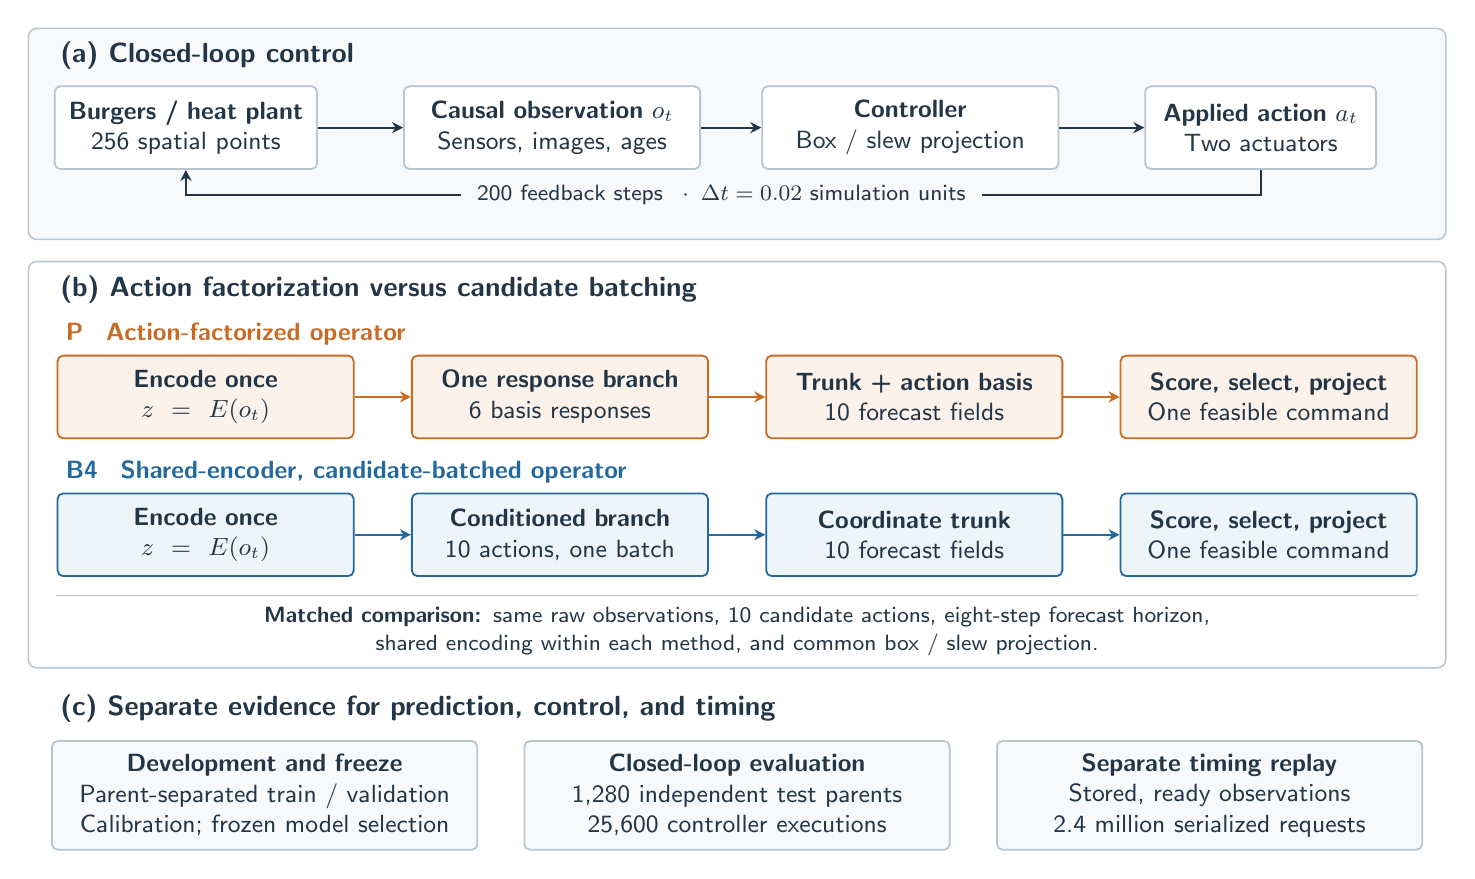
\begin{tikzpicture}[x=1cm,y=-1cm,text=ink,
  box/.style={draw=rule,fill=white,line width=.65pt,rounded corners=2pt,
    align=center,text width=3.48cm,minimum height=1.05cm,inner sep=4pt,
    font=\fontsize{8.7}{11}\selectfont},
  head/.style={anchor=west,font=\bfseries\fontsize{10}{12}\selectfont},
  flow/.style={-{Stealth[length=4pt,width=4pt]},line width=.8pt,draw=ink},
  note/.style={font=\fontsize{8.2}{10}\selectfont,align=center}]

% A: the executed control loop, with a separate, unobstructed feedback path.
\filldraw[fill=panelbg,draw=rule,line width=.55pt,rounded corners=3pt]
  (0,0) rectangle (18,2.68);
\node[head] at (.28,.35) {(a) Closed-loop control};
\node[box,text width=3.05cm] (plant) at (2,1.26)
  {\textbf{Burgers / heat plant}\\256 spatial points};
\node[box] (obs) at (6.65,1.26)
  {\textbf{Causal observation $o_t$}\\Sensors, images, ages};
\node[box] (control) at (11.2,1.26)
  {\textbf{Controller}\\Box / slew projection};
\node[box,text width=2.65cm] (action) at (15.65,1.26)
  {\textbf{Applied action $a_t$}\\Two actuators};
\draw[flow] (plant.east)--(obs.west);
\draw[flow] (obs.east)--(control.west);
\draw[flow] (control.east)--(action.west);
\draw[flow] (action.south)--(15.65,2.12)--(2,2.12)--(plant.south);
\node[note,fill=panelbg,inner xsep=6pt] at (8.8,2.12)
  {200 feedback steps \enspace$\cdot$\enspace $\Delta t=0.02$ simulation units};

% B: parallel, aligned computation stages make the changed operation explicit.
\filldraw[fill=white,draw=rule,line width=.55pt,rounded corners=3pt]
  (0,2.96) rectangle (18,8.12);
\node[head] at (.28,3.32) {(b) Action factorization versus candidate batching};
\node[note,anchor=west,text=orange,font=\bfseries\fontsize{9}{11}\selectfont]
  at (.35,3.88) {P \enspace Action-factorized operator};
\node[box,draw=orange,fill=orangebg] (pe) at (2.25,4.68)
  {\textbf{Encode once}\\$z=E(o_t)$};
\node[box,draw=orange,fill=orangebg] (pr) at (6.75,4.68)
  {\textbf{One response branch}\\6 basis responses};
\node[box,draw=orange,fill=orangebg] (pf) at (11.25,4.68)
  {\textbf{Trunk + action basis}\\10 forecast fields};
\node[box,draw=orange,fill=orangebg] (ps) at (15.75,4.68)
  {\textbf{Score, select, project}\\One feasible command};
\draw[flow,draw=orange] (pe.east)--(pr.west);
\draw[flow,draw=orange] (pr.east)--(pf.west);
\draw[flow,draw=orange] (pf.east)--(ps.west);
\node[note,anchor=west,text=blue,font=\bfseries\fontsize{9}{11}\selectfont]
  at (.35,5.64) {B4 \enspace Shared-encoder, candidate-batched operator};
\node[box,draw=blue,fill=bluebg] (be) at (2.25,6.43)
  {\textbf{Encode once}\\$z=E(o_t)$};
\node[box,draw=blue,fill=bluebg] (br) at (6.75,6.43)
  {\textbf{Conditioned branch}\\10 actions, one batch};
\node[box,draw=blue,fill=bluebg] (bf) at (11.25,6.43)
  {\textbf{Coordinate trunk}\\10 forecast fields};
\node[box,draw=blue,fill=bluebg] (bs) at (15.75,6.43)
  {\textbf{Score, select, project}\\One feasible command};
\draw[flow,draw=blue] (be.east)--(br.west);
\draw[flow,draw=blue] (br.east)--(bf.west);
\draw[flow,draw=blue] (bf.east)--(bs.west);
\draw[draw=rule,line width=.5pt] (.35,7.2)--(17.65,7.2);
\node[note,text width=17cm] at (9,7.66)
  {\textbf{Matched comparison:} same raw observations, 10 candidate actions, eight-step forecast horizon,\\
   shared encoding within each method, and common box / slew projection.};

% C: independent evidence roles, not an implied chain of new experiments.
\node[head] at (.28,8.64) {(c) Separate evidence for prediction, control, and timing};
\node[box,text width=5.12cm,minimum height=1.38cm,fill=panelbg] at (3,9.74)
  {\textbf{Development and freeze}\\Parent-separated train / validation\\Calibration; frozen model selection};
\node[box,text width=5.12cm,minimum height=1.38cm,fill=panelbg] at (9,9.74)
  {\textbf{Closed-loop evaluation}\\1,280 independent test parents\\25,600 controller executions};
\node[box,text width=5.12cm,minimum height=1.38cm,fill=panelbg] at (15,9.74)
  {\textbf{Separate timing replay}\\Stored, ready observations\\2.4 million serialized requests};
\end{tikzpicture}
\end{document}
